% ---------------------------------------------------------------------------------------------------------------- %
% Architecture
% ---------------------------------------------------------------------------------------------------------------- %
\chapter{Architecture} % (fold)
\label{cha:architecture}

% TO-DO
Legacy’s architecture is composed of several entities: the blockchain platform, Legacy’s own infrastructure, an oracle and other third-party services. 
The essential logic of the application is kept inside the blockchain: it is here where the smart contracts that manage user assets are stored and executed. 
Legacy's infrastructure includes the application front ends, as well as a back end to interact with the blockchain, perform heavier computation (\textit{e.g.}, to run the AI engine) and gather additional PoL data.
The oracle is required to provide an interface between the smart contracts and the outside world.
Finally, third-party services can be used for data storage and also to implement plugins for PoL data gathering.
% Third-party services are mostly represented by storage providers but are also useful for providing input data to the PoL engine, whereas most of the application logic would reside in the Blockchain. 
% However, given the current state of maturity of blockchain technologies and related services, some functionalities must be initially implemented using a custom backend as well as third-party infrastructure. As a consequence, Legacy’s architecture is expected to evolve in time, starting from a hybrid architecture and converging towards a fully decentralized architecture.
% In the long-term, the system is expected to evolve autonomously---a design goal that is required in order to minimise trust on the Legacy organization and to guarantee sustained operation in time. Under this scenario, dependence on third-party services (e.g., a storage service such as Filecoin) becomes a less important issue, as we explain later on in this section.


\section{Legacy v1.0 (Memoirs)} % (fold)
\label{sec:legacy_v1_0_memoirs_a_hybrid_architecture}
Legacy v1.0, named \textit{Memoirs}, will be the first stable release of the Legacy Project. This initial version enables secure distribution of memories in the form of digital data, such as pictures, videos, text documents, etc. 
Since blockchain technologies supporting privacy requirements are still evolving, Legacy Memoirs is based on a hybrid architecture, taking advantage of smart contracts but keeping sensible user data outside of the blockchain. In particular, encryption keys will be stored using more traditional systems.
A high-level representation of Legacy Memoirs’ architecture is given in Figure \ref{fig:leg_v1_arch}. Legacy’s own infrastructure and front ends are shown in blue, third-party services in green and the blockchain in red. 

There are two main front ends: a web and a mobile application. These are the main interfaces between the user and the core infrastructure, and provide similar functionalities so that the service can be fully accessed and configured from either.
The web and mobile applications are also employed by the system to obtain PoL data based on user interactions with the service (see also Section~\ref{sec:proof_of_life}).

Legacy’s back end plays different roles. First, it creates smart-contract instances after a user initiates the service and commits a capsule. Second, once a user smart contract is uploaded to the blockchain, the back end sets up an oracle instances that runs periodic calls in order to execute the contract code. And third, it gathers PoL data from external web services and plugins. The user smart contract implements the PoL algorithm that determines if a user is alive or not, schedules subsequent calls from the back end and triggers the distribution of capsules once the PoL engine determines that the user has died. 
Legacy's Memories will implement PoL layers 0 and 1 described in Section~\ref{sec:proof_of_life}.
Memories and capsules will be initially stored using a decentralized, encrypted, blockchain-based, third-party service, which will be backed up using traditional infrastructure.
% Further details are given in Section \ref{sec:data_storage}.
To allow our smart contracts to query the outside world (for instance, for PoL signalling), an Oracle interface is required. Legacy Memoirs will employ an Ethereum-compatible oracle (such us Oraclize\footnote{http://www.oraclize.it/}).

\begin{figure}[h]
  \centering
  \includegraphics[scale=0.4]{fig/architecture_v02_hybrid}
  \caption{Legacy Memoirs architecture.}
  \label{fig:leg_v1_arch}
\end{figure} 

% subsection legacy_v1_0_memoirs_a_hybrid_architecture (end)

\section{Legacy v2.0 (Heritage)} % (fold)
\label{sec:legacy_v2_0_heritage}
Legacy v2.0 \textit{Heritage} will be Legacy’s second stable release. 
One of the key aspects in this version is related to privacy. 
Heritage will implement blockchain privacy features currently under research and development status (see for instance \cite{keep}). The main idea is to minimize trust on Legacy's infrastructure and therefore to store secrets (\textit{e.g.}, users' private keys) securely over the blockchain.
Heritage will also offer the possibility to create legally-bound wills using smart contracts.
In order to facilitate the process of creating valid, legal wills, Heritage also integrates a set of software tools allowing automation of the process, in line with novel advances such as the OpenLaw protocol proposed by Consensys \cite{OpenLaw}.
A major improvement in Legacy's Heritage is the capability to transfer smart property, cryptocurrencies and other blockchain-based assets (though this feature will be subject to the dispositions given by each jurisdiction).
Advancements in blockchain oracle design will also be taken into account in order to further improve and decentralize Legacy's architecture.
Depending on the level of funding available, we expect to implement a first release of Legacy's AI engine, as well as PoL layers 3 and 4.
% subsection legacy_v2_0_heritage_towards_a_fully_decentralized_architecture (end)

\section{Legacy v3.0 (Future): A Decentralized, Autonomous Platform} % (fold)
\label{sec:lgacy_v3_0}
Legacy v3.0 \textit{Future} will pave the way for guaranteeing a long-lasting service capable of evolving over time. Legacy's Future will notably implement the reward and incentive system described in Section~\ref{sub:a_reward_and_incentivisation_system}.
A simplified platform model is shown in Figure~\ref{fig:platform_model}, where in addition to the basic elements included in previous releases, a cross-layer API/SDK module as well as a decentralized governance system is considered.
By leveraging the capabilities provided by the platform, Legacy is expected to become blockchain-agnostic in the long term.
Finally, significant enhancements in both PoL and AI engines are considered to be included.

Table~\ref{tab:releases} summarizes the main features included in each release.

\begin{figure}
	\centering
	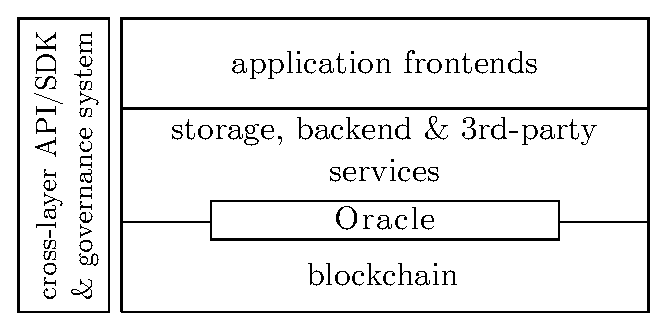
\includegraphics[scale=1.0]{fig/v3_arch.eps}
	\caption{Legacy's platform model}
	\label{fig:platform_model}
\end{figure}
% section lgacy_v3_0_ (end)

% \section{Further Releases} % (fold)
% \label{sec:further_releases}
% % TO-DO


\begin{table}[h]
	\begin{center}		
		{\renewcommand{\arraystretch}{1.3}			
			\begin{tabular}{| c | p{2.5cm} | p{3cm}  | p{4cm} | p{4cm } |}	
		    \hline	
		    \textbf{version}    & \textbf{backend architecture} & \textbf{storage} & \textbf{supported assets} & \textbf{comments} \\ \hline
		    $\alpha / \beta$	& centralized            & centralized      & \textit{memories}         & PoL layers 0--1  \\ \hline		
		    v1.0	            & centralized            & decentralized      & \textit{memories}         & Oracle, PoL layers 0--1 ++  \\ \hline		
		    v2.0 				& decentralized            & decentralized      & \textit{memories}, smart property, cryptocurrencies.  & PoL layers 2 (AI), 3 and 4. Legally-bound SC  \\ \hline		
		    v3.0 				& decentralized, enhanced redundancy & decentralized, enhanced redundancy   & \textit{memories}, smart property, cryptocurrencies   & PoL layers 2--4 ++, AI++, blockchain-agnostic.  \\ \hline
			\end{tabular}				
		}
	\caption{Summary of Legacy's main releases}
	\label{tab:releases}		
	\end{center}
\end{table}
 


% section further_releases (end)

% chapter architecture (end)